\chapter{Papyrus Project Creation}
\label{sec:Appendix1}

In order to implement the application, first of all, a new project has to be created in Eclipse. This project is going to be a Papyrus project (figure \ref{fig:Papyrus Project}).

\begin{figure}
\centering
{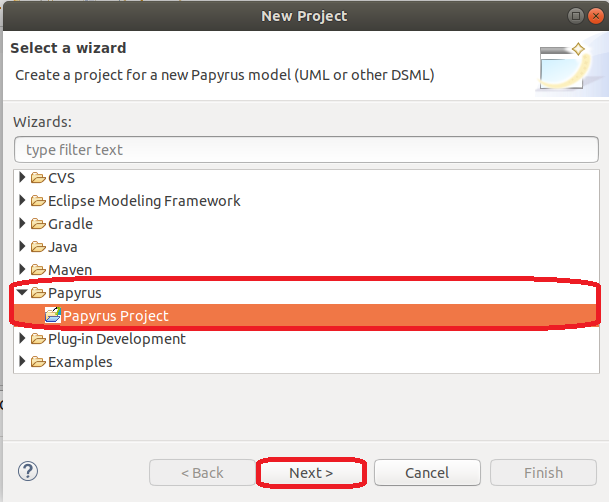
\includegraphics[scale=0.3]{./chapter4/projPapyrus/Selection_001.png}}
\caption{New Papyrus Project}
\label{fig:Papyrus Project}
\end{figure}

The first field that has to be specified is the Architecture Context. Here, the default values are the right ones as an UML model is what is required to implement with Papyrus (figure \ref{fig:Architecture Context}).

\begin{figure}
\centering
{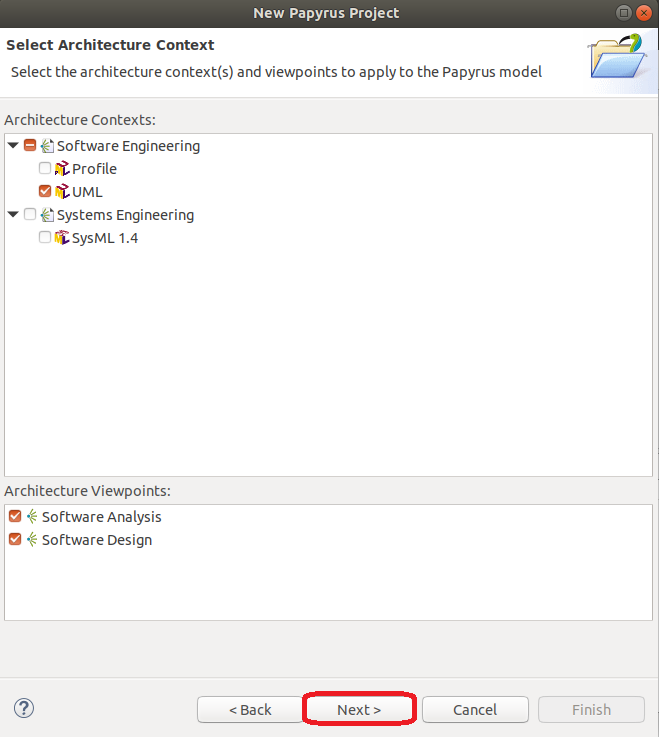
\includegraphics[scale=0.3]{./chapter4/projPapyrus/Selection_002.png}}
\caption{Architecture Context}
\label{fig:Architecture Context}
\end{figure}

After that, the name of the project has to be defined. Due to the fact that it is going to implement an application called Great Seller, the name of the Papyrus project is going to be greatSellerApp (figure \ref{fig:Project Name Definition}).

\begin{figure}
\centering
{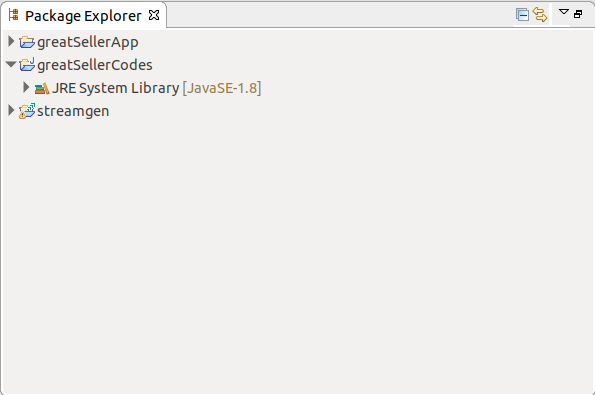
\includegraphics[scale=0.3]{./chapter4/projPapyrus/Selection_003.png}}
\caption{Project Name Definition}
\label{fig:Project Name Definition}
\end{figure}

The next step is to select the representation kind and to choose the StreamGen profile. StreamGen requires Papyrus to make a class diagram representation and, as the StreamGen project is already in the Eclipse workspace, the profile can be found browsing in the workspace (streamgen/profile/StreamUML.profile.uml). As it can be seen in the figure \ref{fig:Representation Kind}.

\begin{figure}
\centering
{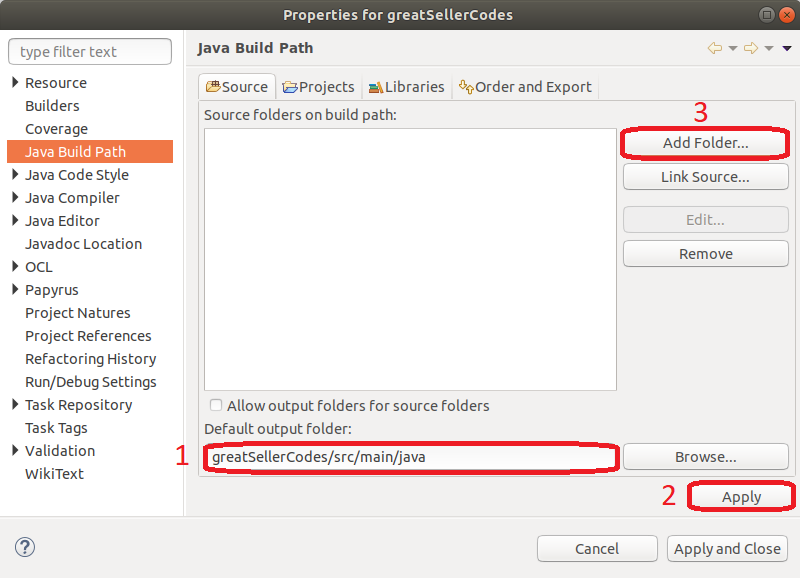
\includegraphics[scale=0.3]{./chapter4/projPapyrus/Selection_004.png}}
\caption{Representation Kind}
\label{fig:Representation Kind}
\end{figure}

Finally, we can finish with the new Papyrus project initialization (figure \ref{fig:Papyrus Project Definition}).

\begin{figure}
\centering
{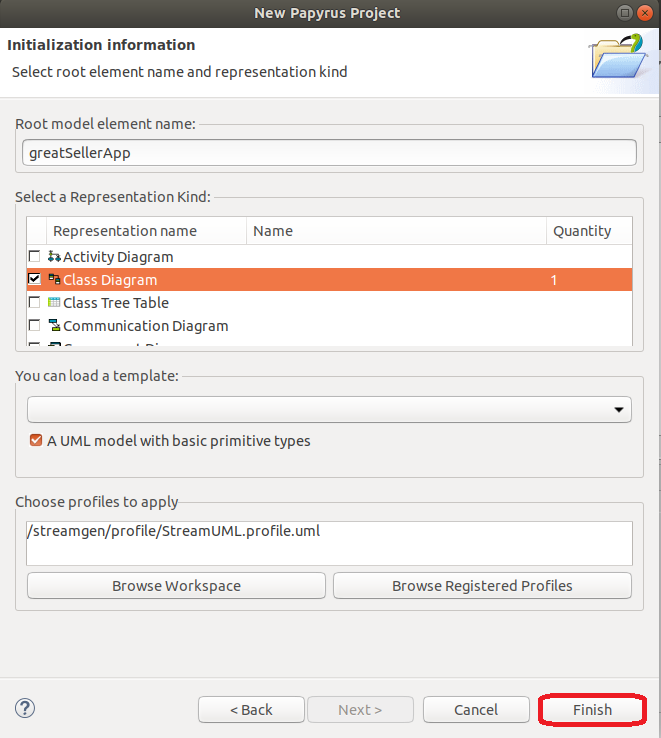
\includegraphics[scale=0.3]{./chapter4/projPapyrus/Selection_005.png}}
\caption{Papyrus Project Definition}
\label{fig:Papyrus Project Definition}
\end{figure}
